% Chapter 1: Introduction

\chapter{Introduction} % Chapter title

\label{ch:introduction} % For referencing the chapter elsewhere, use \autoref{ch:name}

Computer architectures have radically changed in the last 20 years with the introduction of multi-core architectures in almost all areas of computing:
from mobile computing and desktop computers to data centers and high-performance computing.
Furthermore, recently novel types of specialized architectures have been developed featuring large amounts of processing units for dealing with massively data-parallel workloads.
Parallelism and specialization are seen by many computer architects as two crucial answers for overcoming the challenges of increasing performance while at the same time increasing the energy efficiency~\cite{}.

% The development of mainstream programming languages and models have not kept pace with the hardware development.
These modern parallel processors are often still programmed with programming languages developed in the 1980s, like Java or C++, or even older languages like C (from the 1970s) or Fortran (from the 1950s).
These languages have a simplified view of the underlying hardware architecture often more or less directly resembling the Von Neumann architecture.
Multi-core processors are programmed with libraries providing \emph{threads} where the programmer explicitly controls the computations on each core which executes the program in parallel.
This style of programming has turned out to be extremely difficult, as threads running concurrently on distinct cores can modify shared data leading to serious problems like deadlocks, race conditions, and non-determinism.
Even if the programmer develops a correct parallel implementation, optimizing this implementation for modern parallel processors is a challenging task even for experienced programmers.
Due to the lack of better programming systems, programmers are forced to manually develop hardware-specific implementations optimized towards a particular hardware architecture to achieve high performance which limits portability.

This thesis describes our work to address these issues.
In the first part of the thesis we present a high-level programming model and its implementation which is designed to simplify the programming of modern parallel processors, especially systems comprising multiple graphics processing units (\GPUs).
In the second part we discuss a system which generates high-performance code for different modern parallel processors, particularly a multi-core \CPU and two different types of \GPUs, from a single high-level program representation.
In the final part of the thesis we will outline how these two systems can be combined in the future to obtain a programming system which simplifies programming and achieves high-performance on different hardware architectures.

\noindent
We will start our discussion with an introduction on programming modern parallel processors.
From this we will identify the two main challenges we address in this thesis:
the programmability challenge and the performance portability challenge.
We will then list our contributions before presenting the outline for the rest of the thesis.

\section{Multi-Core Processors and their Programming}

% processors become parallel
Traditionally, the performance of microprocessors has been mainly increased by boosting the clock frequency, optimize the execution flow, and improve caches~\cite{Sutter2005}.
This development has drastically changed around 10 years ago, as shown in \autoref{fig:cpuTrend}.
While the number of transistors continues to grow according to Moore's Law~\cite{Moore1998} the clock frequency and power consumption have hit a plateau around 2005.
\begin{figure}
  \centering
  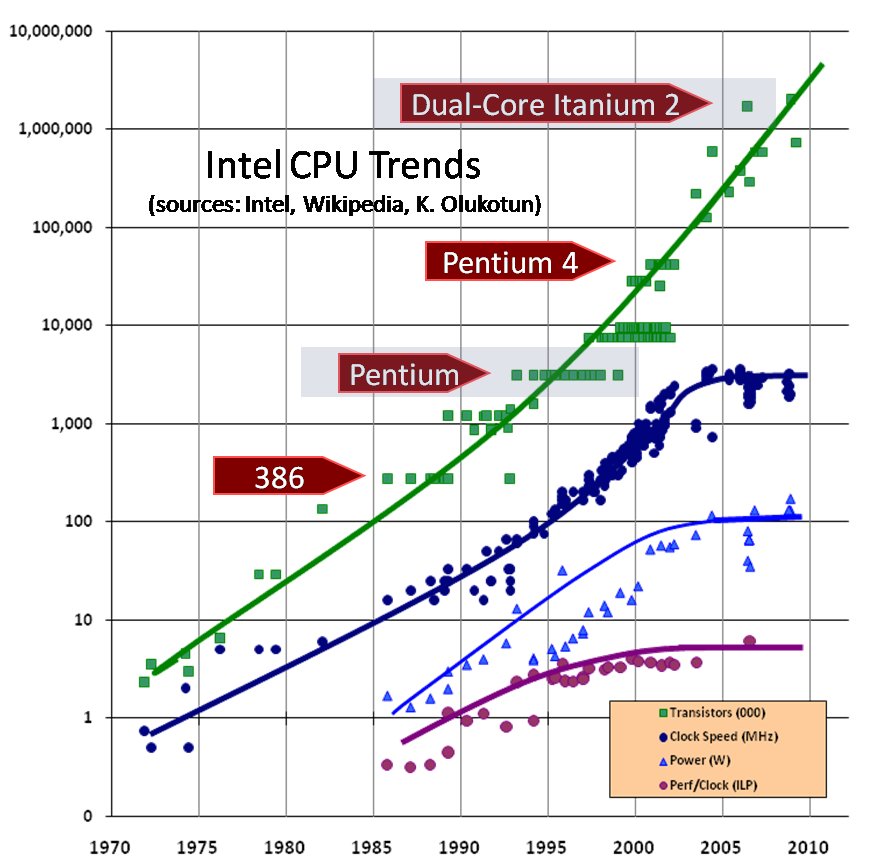
\includegraphics[width=.9\linewidth]{Figures/CPUTrend.png}
  \caption{Development of Intel CPUs over time. Inspired by~\cite{Sutter2005}}
  \label{fig:cpuTrend}
\end{figure} \todo{replace figure}
The reason for this lies in multiple physical effects, especially the physical limit of signal speed and increased heat development, which is mainly due to increased power consumption, both of which limit further increases of the clock frequency.
The predominant answer to this challenge has been the introduction of multiple distinct \emph{cores} which can operate independently and concurrently.
% parallelism is now explicit to the programmer
Parallelism has been exploited in computer architectures for a long time at the bit level and the instruction level, but different than before with the introduction of multiple cores, this new \emph{thread-level parallelism} is explicit to the programmer.
This has profound effects on the design and development of software running on modern multi-core processors.
% programming with threads is a terrible idea
Most programming languages allow programmers to exploit multiple cores by the means of \emph{threads}.
A thread is a sequence of instructions defined by the programmer which can be scheduled by the runtime to be executed on a particular core.
Multiple threads can be executed concurrently and the programmer is responsible to use synchronization primitives, like locks or semaphores, for coordinating the execution of multiple threads.
Programming with threads is widely regarded as extremely difficult~\cite{Lee06} mainly because multiple threads operate on a shared memory region.
Even when programs are constructed carefully subtle problems can arise which are hard to detect but can have severe consequences.
Nevertheless, threads are still the de-facto standard for programming multi-core \CPUs.

\bigskip

\noindent
% still moores law, no dennards scaling
% new hardware trend driven by energy efficiency, specialization, a.k.a heterogeneity, most prominent example: GPUs
While Moore's law still holds and transistor counts increase by further shrinking the transistor size, a related observation, known as Dennard scaling~\cite{DennardRiBaLe1974}, has broken down.
Dennard scaling suggested that power consumption is proportional with the area used for transistors on the chip.
Combined with Moore's law this meant, that the energy efficiency of processors doubled roughly every 18 month.
The primary reason for the breakdown of Dennard scaling around 2005 are physical effects appearing at the small scale of modern transistors, especially current leakage and increased heat development.
This has lead to architectures which particularly focus on their energy efficiency, the most prominent example of such architectures are modern graphics processing units (\GPUs).
Originally developed for accelerating the rendering of complex graphics and 3D scenes, \GPU architectures have been recently generalized to support more types of computations.
Some people refer to this development using the term general-purpose computing on graphics processing units (\GPGPU).

Technically \GPU architectures are multi-core architectures like modern multi-core \CPUs, but each individual core on a \GPU typically has dozens or hundreds of function units which can perform computations in parallel following the single instruction, multiple data (SIMD) principle.
These type of architectures are optimized towards a high throughput of computations, therefore, they focus on performing a large amount of operations in parallel and feature no, or only small, caches to prevent or mitigate latencies of the memory:
if a thread stalls wanting for the memory, another thread takes over and keeps the core busy.
For multi-core \CPUs switching between threads is more expensive, therefore, \CPUs are instead optimized to avoid long latencies when accessing the memory with a deep cache hierarchy and advanced architectural features, like long pipelines and out-of-order execution, all of which is designed to keep each core busy.

\section{The Programmability Challenge}

% programming on the CPU is a nightmare
Developing parallel programs for modern parallel processors is a challenging task.
The dominant approach for programming multi-core \CPUs is using multithreading, \ie, explicitly managing the individual execution paths (called \emph{threads}) in a single program.
Threads communicate via a shared memory, where all threads have the possibility to modify any data item.
This fundamental principle gives the programmer much control over the interaction of the threads but greatly complicates the reasoning about the programs behavior.
The extensive and explicit control directly implies a very low level of abstraction, where the programmer deals with many details of the execution explicitly.
This makes the development of programs using threads complex and certain types of bugs likely like deadlocks and race conditions where the computed result depends on the order the threads are executed in.
This ultimately leads to extensive problems during the development cycle as well as possible non-deterministic and undesirable behavior at runtime.

% not better on the GPU
Programming of \GPUs requires a different programming approach, as it is obviously infeasible to manage thousands of threads explicitly.
\CUDA~\cite{CUDAProgrammingGuide} and \OpenCL~\cite{OpenCL} are the two most popular approaches for programming \GPUs.
Both approaches are quite similar and require the programmer to write a function, called \emph{kernel}, which will be executed in parallel on the \GPU.
The kernel usually contains source code for identifying the thread executing the kernel which is used to coordinate on which data each thread operate on.
While this single program, multiple data (SPMD) programming model makes the management of threads feasible it does not address most problems associated with the low-level programming using threads.
For example, explicit synchronization of threads is still required and problems like deadlocks and race conditions can still easily occur.
Furthermore, \GPU programming currently involves extensive boilerplate code to manage the execution on the \GPU, including the compilation of the kernel (in \OpenCL), transferring data to and from the \GPU, and launching the kernel by explicit specifying the number of threads to be started in parallel.

% There is a challenge: Programmability
All of this leads to our first central research challenge:
can we design a programming approach which significantly raise the level of abstraction and, thus, greatly simplify the development process of parallel applications, without sacrificing high-performance on multi-core \CPUs and \GPUs?
We will underpin the necessity to address this challenge with an extensive study of state-of-the-art \GPU programming using a concrete application example in \autoref{chapter:skelcl}.

In \autoref{part:skelcl} of this thesis, we will introduce, discuss, and evaluate a novel high-level programming model which attempts to address this \emph{challenge of programmability}.

\section{The Performance Portability Challenge}

% extracting performance is hard and not always predictable
Developing functional correct applications for multi-core \CPUs or \GPUs is very challenging as we discussed in the preceding subsection.
Unfortunately, is the development of high-performing optimized applications even more demanding -- even for experienced programmers.
Applying optimizations often requires substantial restructuring of existing code.
Optimizations are often applied ad-hoc following certain ``rules of thumb'' derived from small-scale profiling and experiments as well as previously gained experience.
There exist no widely established approach for performing optimizations more systemically.
Especially, the performance implications of an assumed optimization are currently not predictable:
sometimes supposed optimizations leads to actual slowdowns in certain circumstances.

% compilers do a good job on low-level stuff, but fail for high-level optimizations
Modern optimizing compilers perform very sophisticated low-level optimizations, including various loop optimizations and optimization based on data-flow analysis.
For all these type of optimizations, the compiler first has to recover parts of the high-level program semantics using analysis before applying the optimization.
As these analyses quickly become very complex compilers are ultimately limited in their optimization capabilities.
High-level optimizations which might restructure the entire source code are often out of the reach of low-level compiler optimizations and ,therefore, require explicit and often extensive manual refactoring.
The state-of-the-art optimizing compilers simply are lacking the high-level semantic information necessary for performing these king of optimizations.

% optimizations are hardware-specific
Many optimizations exploit particular hardware-specific features and are, thus, inherently not portable across hardware architectures.
As in current low-level programing model programmers often encode these optimizations directly, programmers are forced with the trade-off of either fully optimize their code for performance -- at the expense of code portability -- or implement a portable version -- at the expense of missing out on the highest performance possible.
Nowadays, programmers often choose a middle ground where introduce conditionals and branches in their code to select optimizations for the given hardware, while maintaining portability.
This, obviously, complicates the development process and decreases maintainability.

% There is a challenge: Performance Protability
This leads to our second central research challenge:
can we design a systematic approach where highly optimized, hardware-specific code is generated from a single high-level program representation?
We will confirm the lack of portability of performance in current state-of-the-art programming approaches using a study comparing optimizations on three different hardware architectures in \autoref{chapter:codeGeneration}.

In \autoref{part:codeGeneration} of this thesis, we will introduce, discuss, and evaluate a novel systematic code generation approach which attempts to address this \emph{challenge of performance portability}.


\section{Contributions of this Thesis}

This thesis makes the following four major contributions:

\subsection*{\hspace{2em}For Addressing the programmability challenge:}

\begin{description}
  \item[A High-level programming model for mutli-\GPU systems]\hfill\\[-1em]
    We present the design and implementation of our high-level programming model \SkelCL for programming multi-\GPU systems.
    \SkelCL offers three high-level features for simplified programming: container data types, algorithmic skeletons, and distributions.
    We discuss our \Cpp library implementation of the \SkelCL programming model which is deeply integrated with modern \Cpp features.
    Finally, we evaluate the level of abstraction and runtime performance of \SkelCL using a set of application studies.

  \item[Two novel algorithmic skeletons]\hfill\\[.25em]
    We introduce two novel algorithmic skeletons specialized towards \emph{allpairs} and \emph{stencil} computations.
    We present their formal definitions and discuss possible use cases in real world applications.
    For the allpairs skeleton we identify and formally define an optimization rule, which enables a more efficient implementation on \GPUs.
    We discuss and evaluate efficient implementations for both skeletons on a multi-\GPU system.
\end{description}

\subsection*{\hspace{2em}For Addressing the performance portability challenge:}

\begin{description}
  \item[A formal system for rewriting pattern-based programs]\hfill\\[-1em]
    We introduce a novel system comprising of set of high-level and low-level patterns along with a set of rewrite rules.
    The rewrite rules express high-level algorithmic and low-level optimization choices which can be systematically applied to transform a program expressed with our functional patterns.
    We proof the soundness of our approach by showing, that applying the rewrite rules does not change the program semantics.

  \item[A code generator offering performance portability]\hfill\\[.25em]
    Based on our formal rewrite system we present a novel code generator which generates from a single pattern-based program highly efficient \OpenCL code for three different hardware architectures:
    one multi-core \CPU and two different \GPUs.
    We discuss the design of our code generator and evaluate the performance of the generated \OpenCL code compared against highly optimized library code.
\end{description}

\section{Outline of this Thesis}
The remainder of this thesis is structured as follows.

\subsection*{Part I -- Introduction}

\paragraph{\autoref{chapter:background}} provides an introduction into the aspects of programming modern multi-core \CPUs and \GPUs.
We will start with the hardware where we mainly focus on \GPUs, discuss their architectures in detail, the state-of-the-art programming approaches, and optimization opportunities.
We will then shift our focus and discuss the algorithmic skeleton parallel programming model including its origins in functional programming.


\subsection*{Part II -- \SkelCL}

\paragraph{\autoref{chapter:skelcl}} addresses the programmability challenge identified in this chapter by introducing our novel \SkelCL high-level programming model targeted towards multi-\GPU systems and its implementation as a \Cpp library.
We will start by further motivating the need for high-level abstractions to simplify the software development process.
Then we present \SkelCL's three high-level features:
1) parallel container data types, 2) algorithmic skeletons, and 3) data distributions.
The combination of these features greatly simplifies the programming of multi-\GPU applications.
Finally, we will discuss the \SkelCL library implementation which is nicely integrated with \Cpp.

\paragraph{\autoref{chapter:skelcl-evaluation}} evaluates the \SkelCL programming model and library using multiple application studies.
We will start with discussing typical benchmark applications like the mandelbrot set computation and benchmarks from linear algebra.
We then continue with discussing more advanced applications from different areas of computing, including image processing, medical imaging, physics, and bioinformatics.
We evaluate the increase of programmability and the performance of \SkelCL compared with implementations written using the state-of-the-art \OpenCL programming approach.


\subsection*{Part III -- Code Generation using Patterns}

\paragraph{\autoref{ch:fifth}} addresses the performance portability challenge identified in this chapter by introducing a novel approach for generating highly optimized hardware-specific code from a single high-level program representation.
We will start the chapter with a study showing that optimizations in \OpenCL are not portable across different hardware architectures.
This emphasizes the motivation for performance portability to preserve maintainability while increase performance and efficiency at the same time.
We continue with discussing the design of our code generation approach consisting of a set of parallel patterns combined with a set of rewrite rules.
The rewrite rules allow to rewrite pattern-based programs without changing their semantics which we will show formally.
Finally, we discuss how the rewrite rules can be systematically applied to optimize pattern-based programs for a particular hardware architecture.

\paragraph{\autoref{ch:sixth}} evaluates our code generation approach using a set of benchmark applications.
We evaluate the performance of the code generated using our approach and compare it against highly tuned library code on three different hardware architectures.

\subsection*{Part IV -- Summary \& Conclusions}

\paragraph{\autoref{ch:seventh}} summarizes Part II and Part II and describes their relation.
We will discuss how \SkelCL, presented in Part II, could be combined in the future with the code generator, presented in Part III, to obtain a system offering both high-level abstractions to simplify programming and portable high-performance on different hardware architectures.

\paragraph{\autoref{ch:eighth}} concludes the thesis with a comparison against related work and discussing possible future extensions of our research.

